\chapter{Implementasi dan Pengujian}
\label{chap:implementasiPengujian}

Bab ini terdiri atas dua bagian, yaitu Implementasi Perangkat Lunak dan Pengujian Perangkat Lunak. Bagian implementasi berisi penjelasan lingkungan pengembangan perangkat lunak dan hasil implementasi. Sedangkan bagian pengujian berisi hasil pengujian fungsional dan eksperimental terhadap perangkat lunak yang telah dibangun.

\section{Implementasi}
\label{sec:implementasi}

\subsection{Lingkungan Implementasi}
\label{sec:lingkungan_implementasi}
Implementasi perangkat lunak ini dilakukan di komputer dengan spesifikasi sebagai berikut:
\begin{enumerate}
	\item Processor: 1.6 GHz
	\item RAM: 4 GB 1600 MHz DDR3
	\item Sistem Operasi: OS X Yosemite version 10.10.5
	\item Versi Java: 1.8.0\_51
\end{enumerate}

\textbf{Server MAMP}\\
Server yang digunakan untuk menjalankan aplikasi KIRI dalam bahasa PHP adalah server MAMP. MAMP adalah kumpulan dari perangkat lunak \textit{open-source} dan bebas komersial yang digunakan secara bersamaan untuk menjalankan situs web dinamis pada sistem operasi Apple Macintosh \cite{mamp}. MAMP adalah singkatan dari:
\begin{enumerate}
	\item Mac OS X, yaitu sistem operasi yang digunakan
	\item Apache, yaitu web server yang digunakan untuk menjalankan web
	\item MySQL, yaitu manajemen basisdata yang digunakan pada web
	\item PHP, Perl, atau Phyton, yaitu bahasa pemrograman yang digunakan untuk pengembangan web.
\end{enumerate}

\subsection{Hasil Implementasi}
Hasil implementasi berupa aplikasi berbasis web yang menggunakan Play Framework. Aplikasi dapat diakses pada jaringan lokal dengan URL \url{http://localhost:9000}. Aplikasi KIRI terdiri dari satu halaman utama. Halaman utama KIRI, pengguna dapat melakukan pencarian rute KIRI dengan masukan nama tempat atau masukan berupa klik pada peta yang disediakan pada halaman utama KIRI (Gambar \ref{fig:5_KIRI_main}).
\begin{itemize}
	\item Pencarian rute dan alternatif pencarian rute\\
	Setelah memberikan masukan untuk pencarian rute, jika terdapat pencarian rute, maka hasil rute dan/atau hasil alternatif rute akan ditampilkan pada halaman utama KIRI serta menggambarkan hasil rute pada peta. Hasil pencarian rute dapat dilihat pada gambar \ref{fig:5_KIRI_find}, sedangkan hasil pencarian rute alternatif dapat dilihat pada gambar \ref{fig:5_KIRI_find_alternate}.
	\item Tidak ada rute\\
	Setelah memberikan masukan untuk pencarian rute, jika tidak terdapat pencarian rute, maka akan menampilkan pesan pada pengguna (Gambar \ref{fig:5_KIRI_not_found}).
\end{itemize}

\begin{figure}[H]
	\centering
	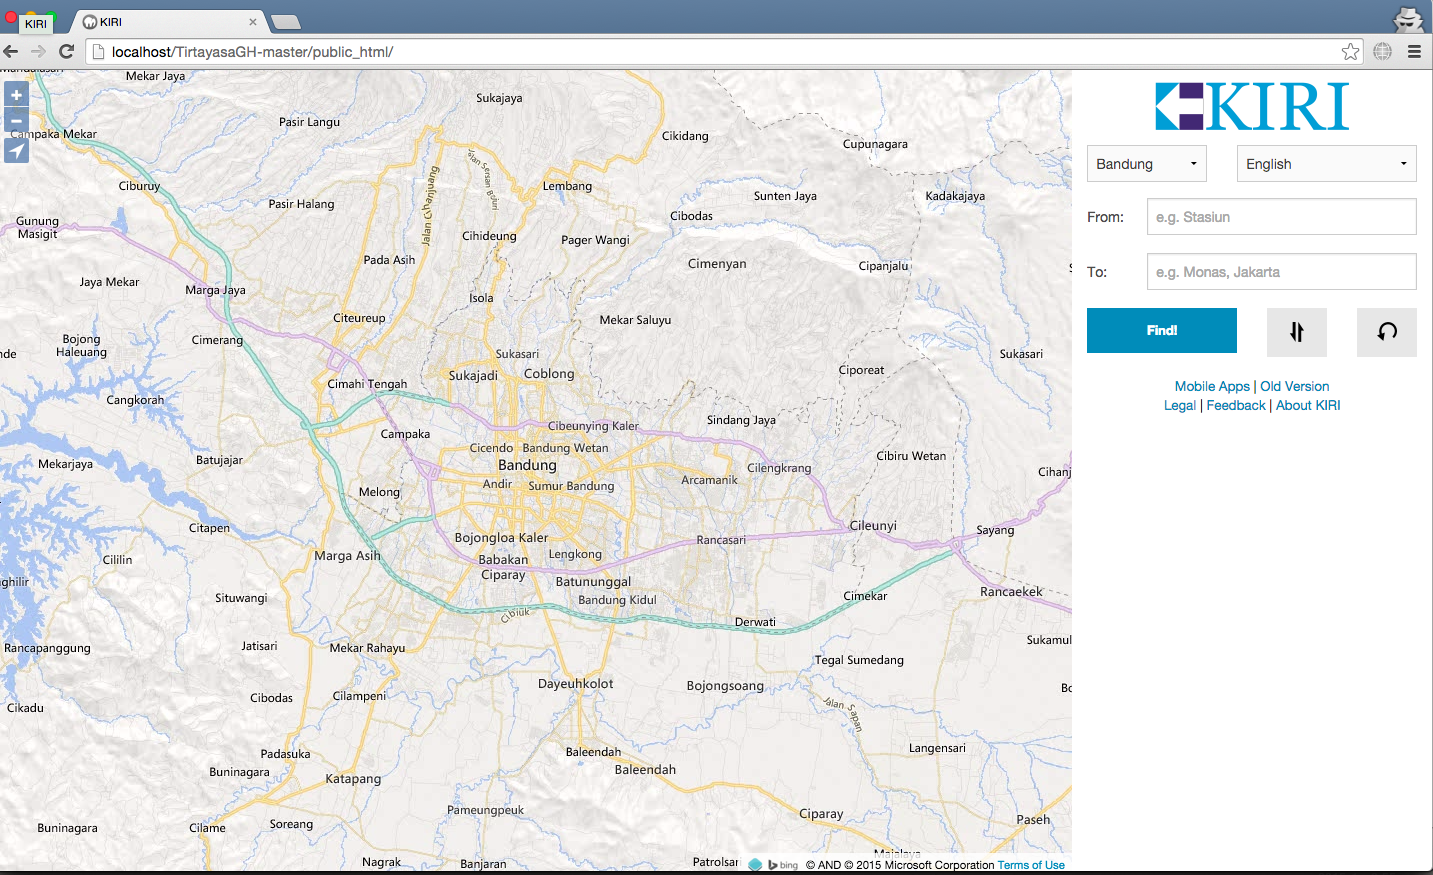
\includegraphics[scale=0.3]{Gambar/KIRI-main-5}
	\caption{Halaman Utama KIRI} 
	\label{fig:5_KIRI_main}
\end{figure}


\begin{figure}[H]
	\centering
	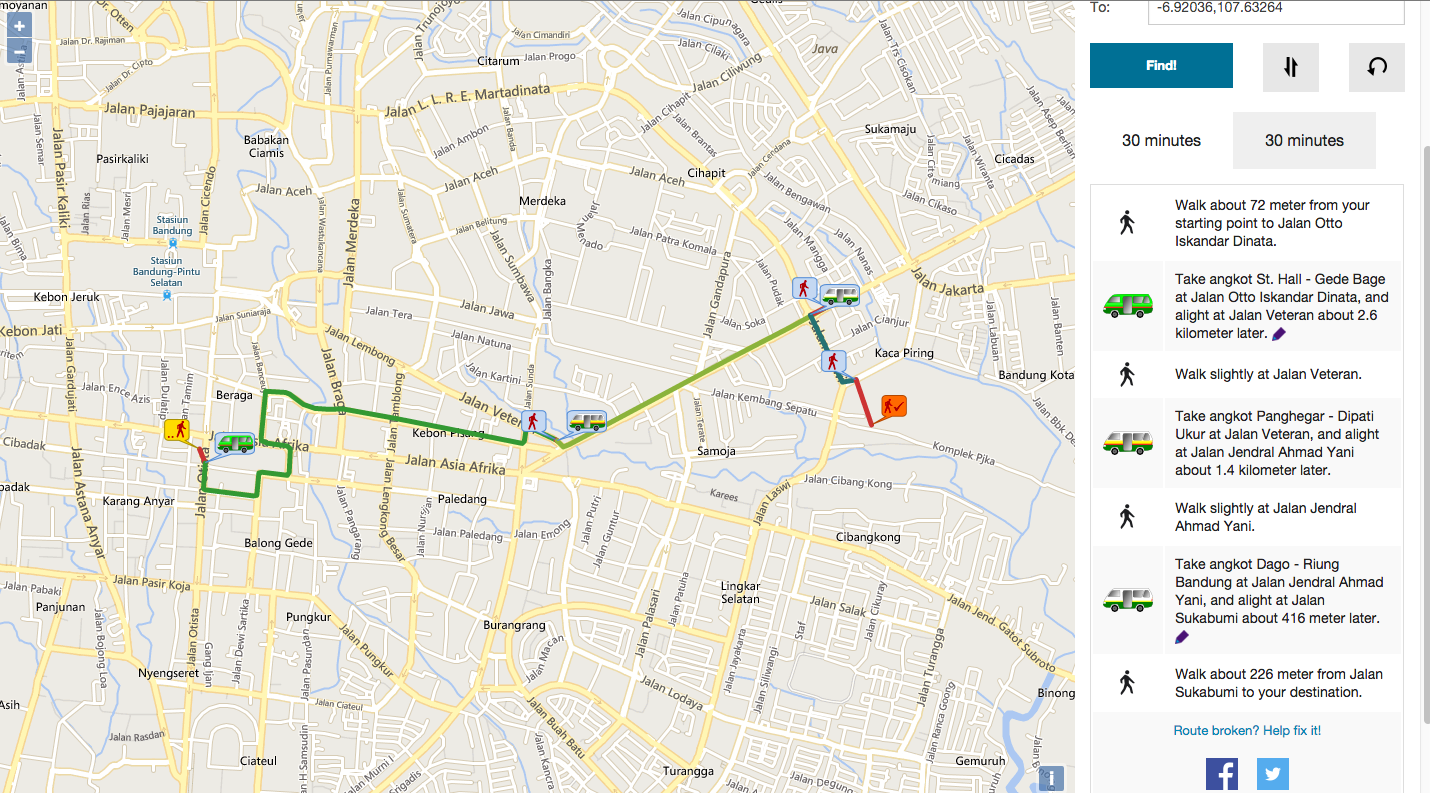
\includegraphics[scale=0.3]{Gambar/KIRI-find}
	\caption{Contoh Pencarian Rute pada KIRI} 
	\label{fig:5_KIRI_find}
\end{figure}

\begin{figure}[H]
	\centering
	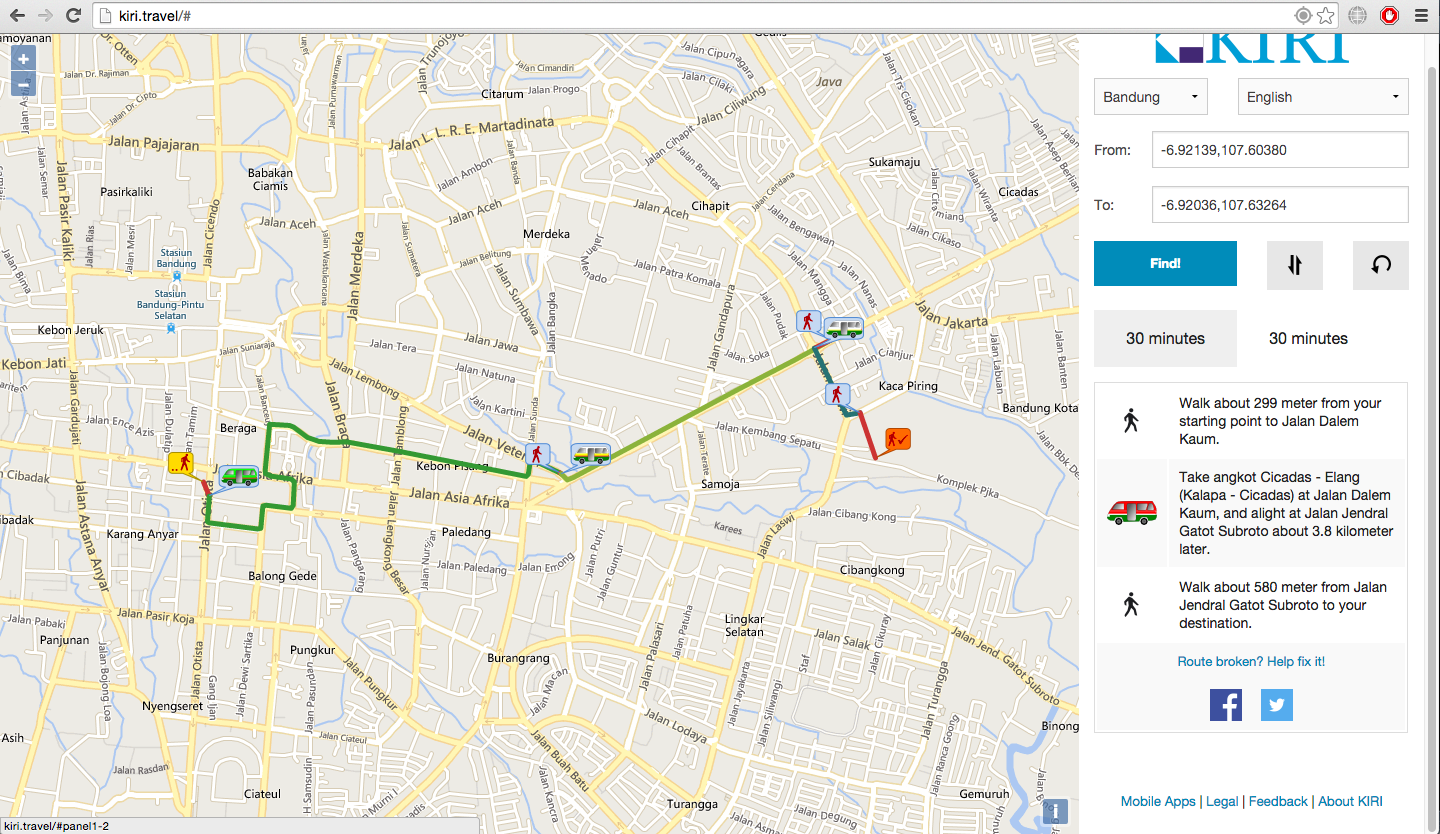
\includegraphics[scale=0.3]{Gambar/KIRI-find-alternate}
	\caption{Contoh Rute Alternatif pada KIRI} 
	\label{fig:5_KIRI_find_alternate}
\end{figure}

\begin{figure}[H]
	\centering
	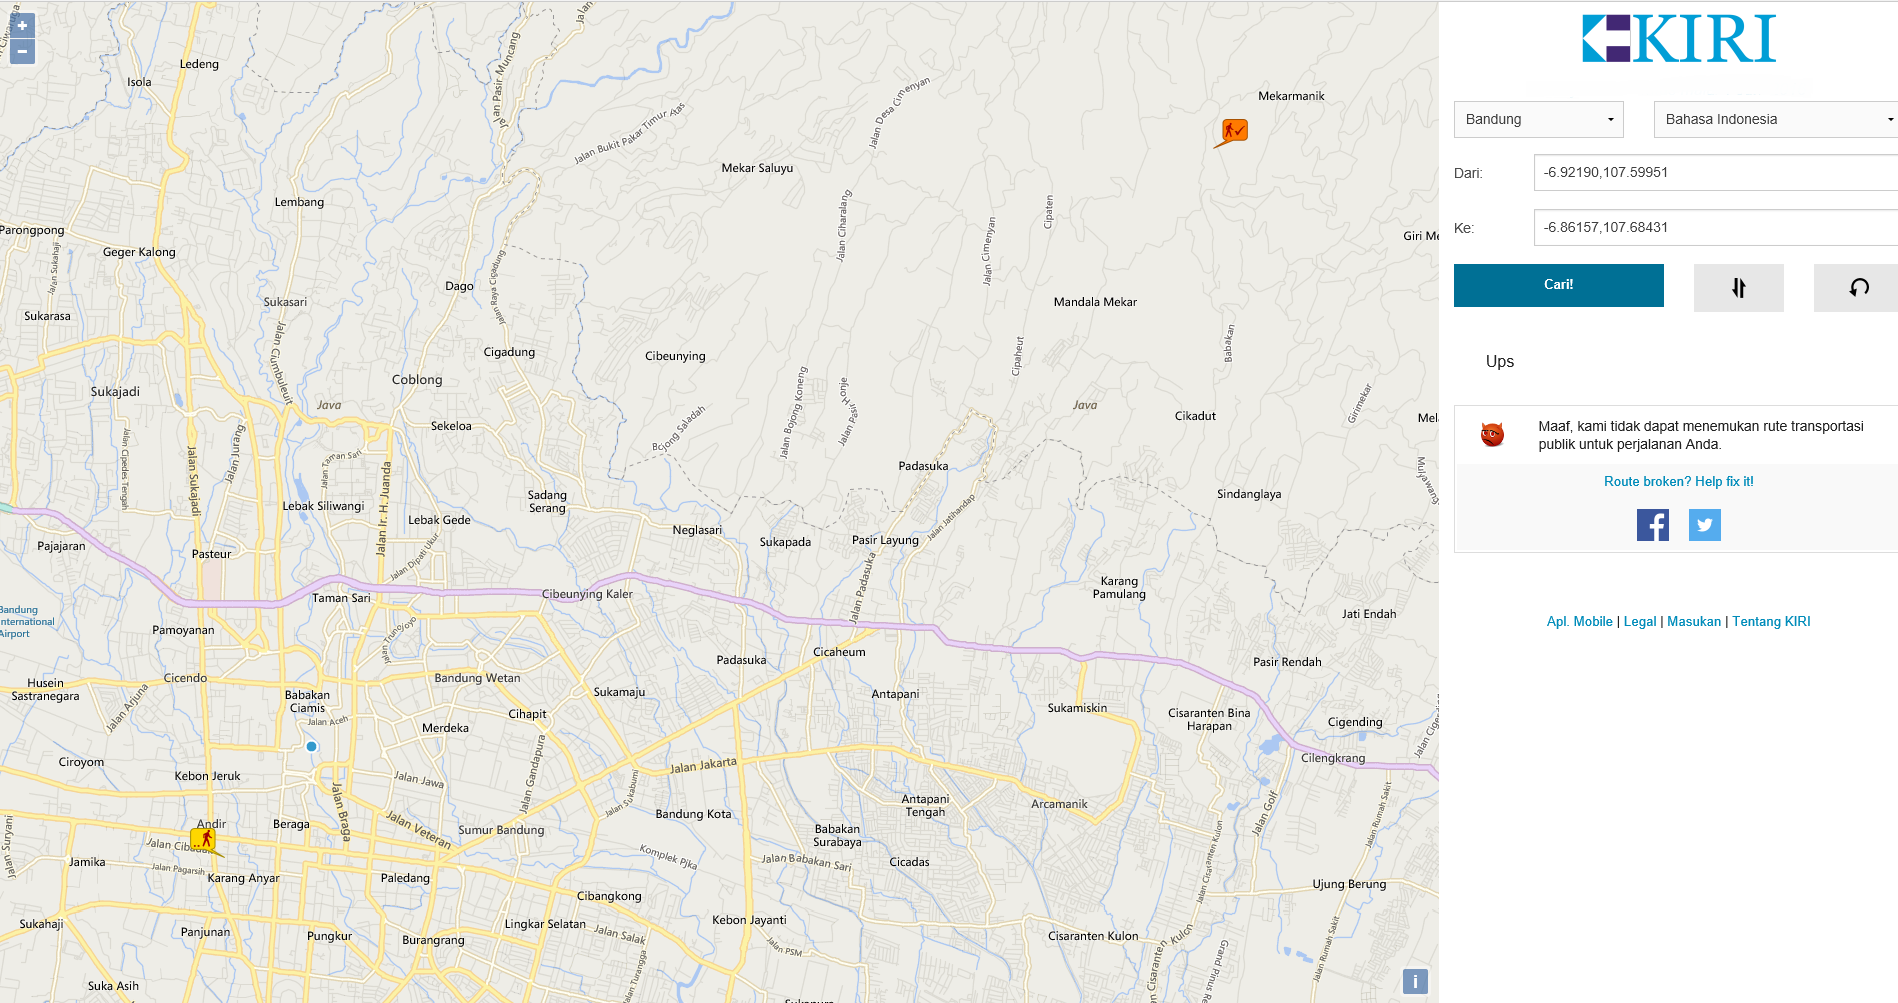
\includegraphics[scale=0.3]{Gambar/KIRI-notfound}
	\caption{Menampilkan pesan tidak ada rute pada pengguna} 
	\label{fig:5_KIRI_not_found}
\end{figure}

\section{Pengujian}
\subsection{Pengujian Fungsional}

Pengujian fungsional dilakukan untuk mengetahui kesesuaian reaksi perangkat lunak dengan reaksi yang diharapkan berdasarkan aksi pengguna terhadap perangkat lunak. Pengujian ini dilakukan pada berbagai sistem yaitu Windows dan MacOS dengan hasil yang sama. Terdapat sembilan tes kasus yang diujikan, detail serta hasilnya dapat dilihat pada Tabel \ref{table:hasilFungsional}.
			
\begin{table}[H]
	\centering
	\caption{Tabel Pengujian Fungsional}
		\begin{tabular}{|p{0.25cm}| p{3.5cm}| p{7cm}| p{2.5cm}|} \hline
		No.	&	Aksi Pengguna	&	Reaksi yang diharapkan	&	Reaksi Perangkat Lunak \\ \hline
		1 & Pengguna menjalankan aplikasi & Halaman utama ditampilkan & Sesuai \\ \hline
2 & Pengguna memilih kota yang ingin ditampilkan & Memperbarui peta dengan kota yang dipilih & Sesuai \\ \hline
3 & Pengguna memilih bahasa yang ingin ditampilkan & Memperbarui tampilan dengan bahasa yang dipilih & Sesuai \\ \hline
4 & Pengguna melakukan klik pada peta & \textit{Marker} muncul dari titik yang diklik oleh pengguna dan titik koordinat muncul pada \textit{textfield} tempat asal dan/atau tujuan & Sesuai \\ \hline
5 & Pengguna memilih tombol Swap & Masukan pengguna pada \textit{textfield} tempat awal dan tujuan ditukar & Sesuai \\ \hline
6 & Pengguna memilih tombol Reset & Memperbarui halaman utama menjadi semula & Sesuai \\ \hline
7 & Pengguna memilih tombol Find & Hasil pencarian rute muncul beserta alternatifnya (jika ada) & Sesuai, namun JSON yang dihasilkan mempunyai urutan \textit{key} yang berbeda. Hal ini tidak mengubah arti pesan yang dikirim karena JSON dapat diakses dengan mengirimkan \textit{parameter key}. \\ \hline
8 & Pengguna memasukkan nama tempat pada \textit{textfield} tempat asal dan/atau tujuan & Sugesti nama tempat muncul pada masing-masing \textit{textfield} dan menampilkan hasil pencarian beserta alternatifnya (jika ada) & Sesuai \\ \hline
9 & Pengguna memilih hasil pencarian rute alternatif & Hasil pencarian rute alternatif muncul dan memperbarui peta dengan hasil pencarian rute alternatif & Sesuai \\ \hline
		
		\end{tabular}
	\label{table:hasilFungsional}
\end{table}


\subsection{Pengujian Eksperimental}

Pengujian eksperimental dilakukan untuk membandingkan perbedaan waktu eksekusi dari aplikasi KIRI (PHP) dengan aplikasi KIRI (Play Framework). Pengujian eksperimental mengambil lima tes kasus dan masing-masing kasus diambil empat kali pengujian. Kelima kasus tersebut menggunakan parameter tempat asal dan tujuan yang sama, menggunakan koneksi internet yang sama, dan menggunakan \textit{web browser} yang sama. Waktu diambil menggunakan Chrome DevTools dan menghitung waktu eksekusi dalam memuat halaman web untuk setiap kasus. Pengujian ini dilakukan pada sistem MacOS. Hasil pengujian dapat dilihat pada tabel  \ref{table:hasilEksperimental} dan grafik \ref{fig:5_grafik_eksperimental}.
			
\begin{table}[H]
	\centering
	\caption{Tabel Pengujian Eksperimental}
	\scalebox{0.8}{
		\begin{tabular}{|l|l|c|c|c|c|c|}
\hline
No. & \multicolumn{1}{c|}{Aksi} & \multicolumn{5}{c|}{PHP} \\ \hline
\multicolumn{2}{|l|}{} & \begin{tabular}[c]{@{}c@{}}Waktu \\ eksekusi \\ pertama\\(detik)\end{tabular} & \begin{tabular}[c]{@{}c@{}}Waktu\\ eksekusi\\ kedua\\(detik)\end{tabular} & \begin{tabular}[c]{@{}c@{}}Waktu\\ eksekusi\\ ketiga\\(detik)\end{tabular} & \begin{tabular}[c]{@{}c@{}}Waktu\\ eksekusi\\ keempat\\(detik)\end{tabular} & \begin{tabular}[c]{@{}c@{}}Rata-\\ rata\\(detik)\end{tabular} \\ \hline
1. & Pengguna akses halaman utama KIRI & 1.00 & 0.89 & 0.87 & 1.57 & 1.08 \\ \hline
2. & Pengguna mencari rute dengan memasukkan nama tempat & 4.12 & 3.97 & 3.55 & 2.54 & 3.55 \\ \hline
3. & Pengguna mencari rute dengan klik pada peta & 3.69 & 3.16 & 4.04 & 5.78 & 4.17 \\ \hline
4. & Pengguna mengirimkan request dengan mode sama dengan `findroute' & 1.17 & 2.92 & 3.22 & 3.36 & 2.67 \\ \hline
5. & Pengguna mengirimkan request dengan mode sama dengan `searchplace' & 1.14 & 0.78 & 0.52 & 1.16 & 0.90 \\ \hline
\end{tabular}
}
	\label{table:hasilEksperimental}
\end{table}

\begin{table}[H]
	\centering
	\scalebox{0.8}{
		\begin{tabular}{|l|l|c|c|c|c|c|}
\hline
No. & \multicolumn{1}{c|}{Aksi} & \multicolumn{5}{c|}{Play Framework} \\ \hline
\multicolumn{2}{|l|}{} & \begin{tabular}[c]{@{}c@{}}Waktu\\ eksekusi\\ pertama\\(detik)\end{tabular} & \begin{tabular}[c]{@{}c@{}}Waktu\\ eksekusi\\ kedua\\(detik)\end{tabular} & \begin{tabular}[c]{@{}c@{}}Waktu\\ eksekusi\\ ketiga\\(detik)\end{tabular} & \begin{tabular}[c]{@{}c@{}}Waktu\\ eksekusi\\ keempat\\(detik)\end{tabular} & \begin{tabular}[c]{@{}c@{}}Rata-\\ rata\\(detik)\end{tabular} \\ \hline
1. & Pengguna akses halaman utama KIRI & 1.51 & 1.58 & 1.67 & 1.59 & 1.59 \\ \hline
2. & Pengguna mencari rute dengan memasukkan nama tempat & 2.08 & 1.15 & 2.54 & 2.74 & 2.13 \\ \hline
3. & Pengguna mencari rute dengan klik pada peta & 1.98 & 4.24 & 3.22 & 2.76 & 3.05 \\ \hline
4. & Pengguna mengirimkan request dengan mode sama dengan `findroute' & 3.63 & 2.15 & 2.96 & 1.41 & 2.54 \\ \hline
5. & Pengguna mengirimkan request dengan mode sama dengan `searchplace' & 0.72 & 0.1 & 1.38 & 0.88 & 0.77 \\ \hline
\end{tabular}
}
\end{table}

\begin{figure}[H]
	\centering
	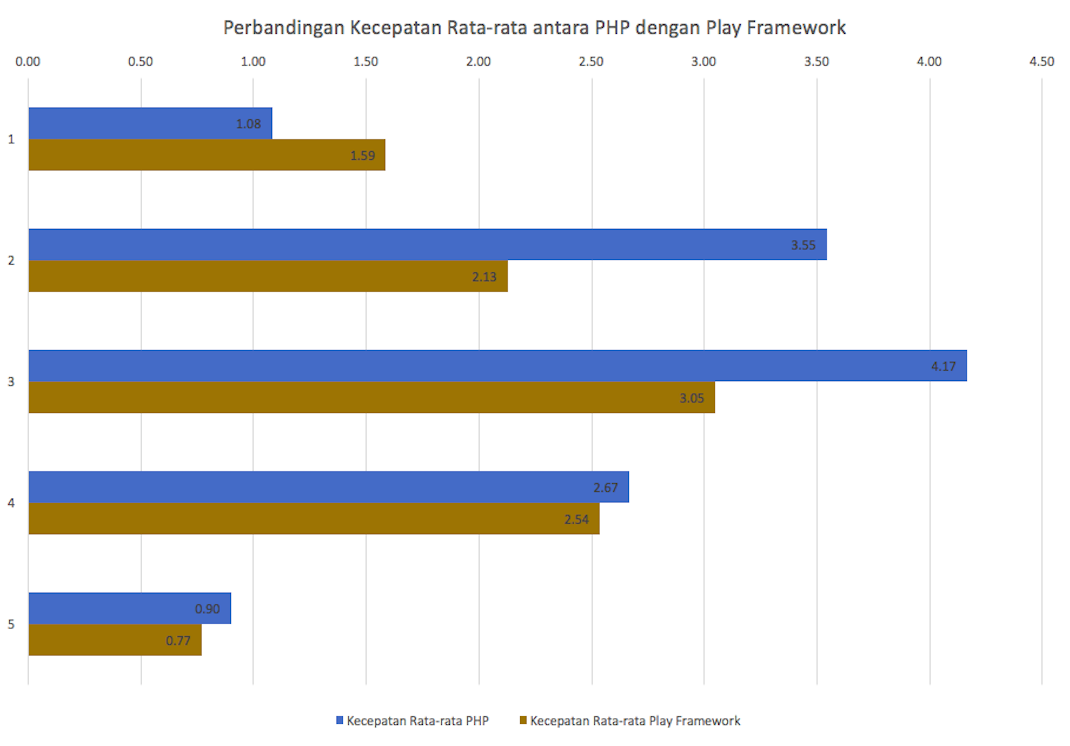
\includegraphics[scale=0.4]{Gambar/grafik-eksperimental}
	\caption{Grafik Perbandingan Kecepatan} 
	\label{fig:5_grafik_eksperimental}
\end{figure}

Dari hasil dan grafik pengujian eksperimental, didapat kesimpulan bahwa waktu eksekusi \play lebih cepat dalam memuat konten yang dinamis. Konten dinamis termasuk dengan struktur data dalam memuat konten dinamis tersebut. Sedangkan untuk konten statis, waktu eksekusi \play lebih lambat dibandingkan dengan PHP. Konten statis yang dimaksud adalah memuat konten tanpa melalui proses terlebih dahulu, misalnya gambar, JavaScript, dan Stylesheet pada aplikasi.